% This work is made available under the terms of the
% Creative Commons Attribution-ShareAlike 3.0 license, 
% http://creativecommons.org/licenses/by-sa/3.0/. 
%
% Version: $Revision: 3363 $

\documentclass[a4paper]{book}

\usepackage{wrapfig}
\usepackage{graphicx}
\usepackage{hyperref}
\usepackage{multirow}
\usepackage{scalefnt}
\usepackage{tikz}
\usepackage{varwidth}

% watermark -- for draft stage
\usepackage[firstpage]{draftwatermark}
\SetWatermarkLightness{0.9}
\SetWatermarkScale{5}

% Copyright (c) 2009 by the University of Waikato, Hamilton, NZ. 
% This work is made available under the terms of the 
% Creative Commons Attribution-ShareAlike 4.0 license,
% http://creativecommons.org/licenses/by-sa/4.0/.
%
% Version: $Revision: 5479 $

\newenvironment{tight_itemize}{
\begin{itemize}
  \setlength{\itemsep}{1pt}
  \setlength{\parskip}{0pt}
  \setlength{\parsep}{0pt}}{\end{itemize}
}

\newenvironment{tight_enumerate}{
\begin{enumerate}
  \setlength{\itemsep}{1pt}
  \setlength{\parskip}{0pt}
  \setlength{\parsep}{0pt}}{\end{enumerate}
}

% if you just need a simple heading
% Usage:
%   \heading{the text of the heading}
\newcommand{\heading}[1]{
  \vspace{0.3cm} \noindent \textbf{#1} \newline
}

\newcommand{\icon}[1]{\tikz[baseline=-3pt]\node[inner sep=0pt,outer sep=0pt]{\includegraphics[height=1.1em]{#1}};}


\title{
  \textbf{ADAMS} \\
  {\Large \textbf{A}dvanced \textbf{D}ata mining \textbf{A}nd \textbf{M}achine
  learning \textbf{S}ystem} \\
  {\Large Module: adams-video} \\
  \vspace{1cm}
  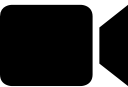
\includegraphics[width=2cm]{images/video-module.png} \\
}
\author{
  Peter Reutemann \\
  Steven Brown
}

\setcounter{secnumdepth}{3}
\setcounter{tocdepth}{3}

\begin{document}

\begin{titlepage}
\maketitle

\thispagestyle{empty}
\center
\begin{table}[b]
	\begin{tabular}{c l l}
		\parbox[c][2cm]{2cm}{\copyright 2015-2016} &
		\parbox[c][2cm]{5cm}{
\includegraphics[width=5cm]{images/coat_of_arms.pdf}} \\
	\end{tabular}
	
\includegraphics[width=12cm]{images/cc.png} \\
\end{table}

\end{titlepage}

\tableofcontents
\listoffigures
%\listoftables

%%%%%%%%%%%%%%%%%%%%%%%%%%%%%%%%%%%
\chapter{Flow}
The video module offers some actors for basic video display and processing support.

\noindent Available standalones:
\begin{tight_itemize}
    \item \textit{RecordingSetup} -- configures a recording setup (sound/screen/webcam).
    \item \textit{StartRecording} -- starts a defined recording setup.
    \item \textit{StopRecording} -- stops a defined recording setup.
\end{tight_itemize}

\noindent Available sources:
\begin{tight_itemize}
    \item \textit{ListWebcams} -- lists the names of all available webcams
    attached to the computer\footnote{adams-video-list\_webcams.flow}.
    \item \textit{WebcamImage} -- outputs images from the selected webcam
    attached to the computer\footnote{adams-video-webcam.flow}.
    \item \textit{WebcamInfo} -- outputs images from the selected webcam
    \footnote{adams-video-webcam\_info.flow}.
\end{tight_itemize}

\noindent Available transformers:
\begin{tight_itemize}
	\item \textit{AddTrailBackground} -- adds a image as trail
	background\footnote{adams-video-track\_objects-predefined3.flow}
	\item \textit{AddTrailStep} -- adds an additional step to the trail
	passing through\footnote{adams-video-track\_objects-predefined3.flow}.
	\item \textit{ExtractTrackedObject} -- extracts a tracked
	object in an image and forwards it as new image.
	container\footnote{adams-video-track\_objects-user\_selected\_object.flow}.
	\item \textit{GetTrailBackground} -- retrieves the trail background image, if any.
	\item \textit{MjpegImageSequence} -- generates an image sequence
	from MJPEG movies, one frame at a time\footnote{adams-video-play\_mjpeg\_video.flow}.
	\item \textit{MovieImageSampler} -- extracts images from a movie using a sampling algorithm.
	\item \textit{MovieImageSequence} -- generates an image sequence
	from movies, one frame at a time (uses Xuggle\cite{xuggle}\footnote{adams-video-play\_mp4\_video.flow}).
	\item \textit{MovieInfo} -- extracts information from movie files\footnote{adams-video-movie\_info.flow}.
	\item \textit{TrackObjects} -- tracks objects in images sequences,
	e.g., from movies\footnote{adams-video-track\_objects-predefined.flow, adams-video-track\_objects-predefined2.flow}.
	\item \textit{TrailFileReader} -- reads a trail from disk.
	\item \textit{TrailFileWriter} -- writes a trail to disk\footnote{adams-video-track\_objects-predefined3.flow}.
	\item \textit{TrailFilter} -- applies a filter to the trail passing through.
	\item \textit{TransformTrackedObject} -- transforms a tracked
	object in an image with a callable transformer, e.g., for blurring a
	face\footnote{adams-video-track\_objects-predefined2.flow}.
\end{tight_itemize}

\noindent Available sinks:
\begin{tight_itemize}
  \item \textit{AnimatedGifFileWriter} -- generates an animated GIF from
  an array of image files or images.
  \item \textit{FFmpeg} -- actor for processing videos using
  ffmpeg\cite{ffmpeg}\footnote{adams-video-ffmpeg.flow}.
  \item \textit{TrailDisplay} -- displays trail objects\footnote{adams-video-display\_trail.flow, adams-video-track\_objects-predefined3.flow}.
\end{tight_itemize}

\noindent Available conversions:
\begin{tight_itemize}
  \item \textit{QuadrilateralLocationCenter} -- outputs a Point2D object that
  is the center of the rectangle surrounding the quadrilateral coordinates.
  \item \textit{QuadrilateralLocationToString} -- turns the quadrilateral
  coordinates into a string.
  \item \textit{StringToQuadrilateralLocation} -- turns a string into quadrilateral
  locations.
\end{tight_itemize}

%%%%%%%%%%%%%%%%%%%%%%%%%%%%%%%%%%%
\chapter{Tools}

\section{Trail viewer}
The \textit{Trail viewer} is a simple tool for viewing trails of objects that
have been tracked using a flow. It can be used to apply filters to trails
and save those trails back to disk. Figure \ref{trail_viewer} shows a screenshot.

\begin{figure}[htb]
  \centering
  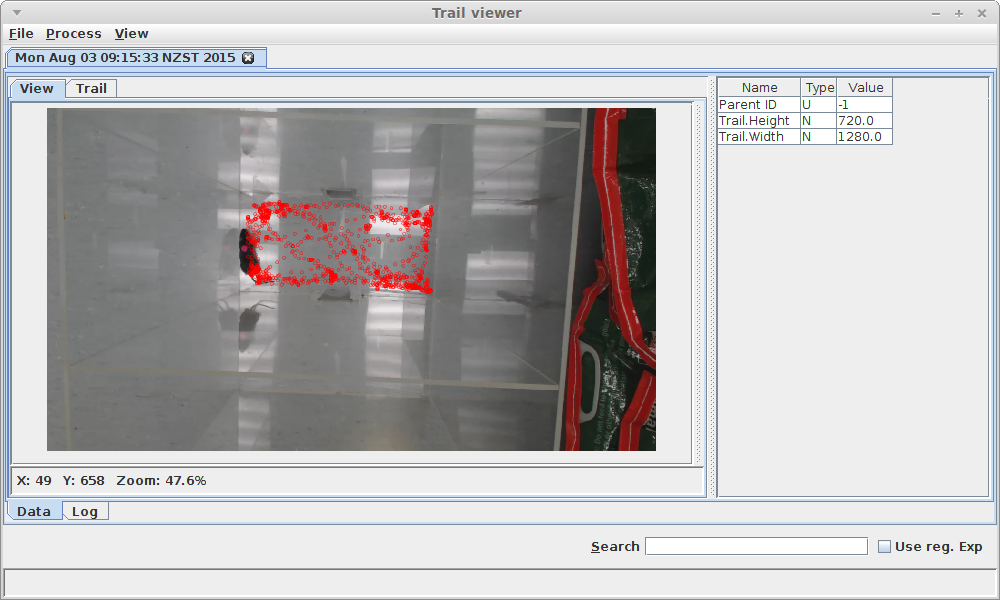
\includegraphics[width=12.0cm]{images/trail_viewer.png}
  \caption{Trail viewer displaying a mice trail overlayed on a background image.}
  \label{trail_viewer}
\end{figure}

\section{vlcj Video Player}
A simple video player used to play video or audio files in real time. To use this tool, or any other tools
that incorpoate it, a user must have VLC player installed on their computer.
The bitness of the VLC player install and the Java install must be the same, that is
they must both either be 32 bit installs or 64 bit installs. Figure \ref{VideoPlayerInUse} shows the player
being used.

 \begin{figure}[htb]
   \centering
   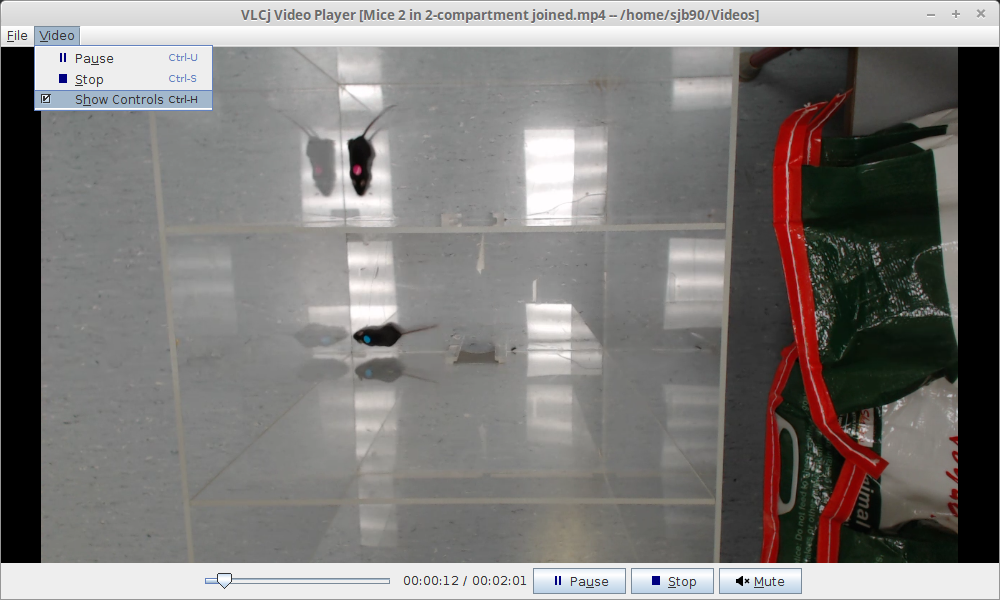
\includegraphics[width=12.0cm]{images/video_player_in_use.png}
   \caption{Video Player in use.}
   \label{VideoPlayerInUse}
 \end{figure}

\section{Video Annotator}
The \textit{Video Annotator} is a tool for creating annotations for a video. A user can
create their own personalized key shortcuts which they can then use to add annotations at a given time stamp.
The annotations can be exported for use in a spreadsheet or other post processing. Figure \ref{annotator_in_use}
shows a screen shot. The video annotator incorporates the vlcj Video Player and has the same requirements, i.e. --- VLC
player must be installed and the bitness of the installs must match.

\begin{figure}[htb]
  \centering
  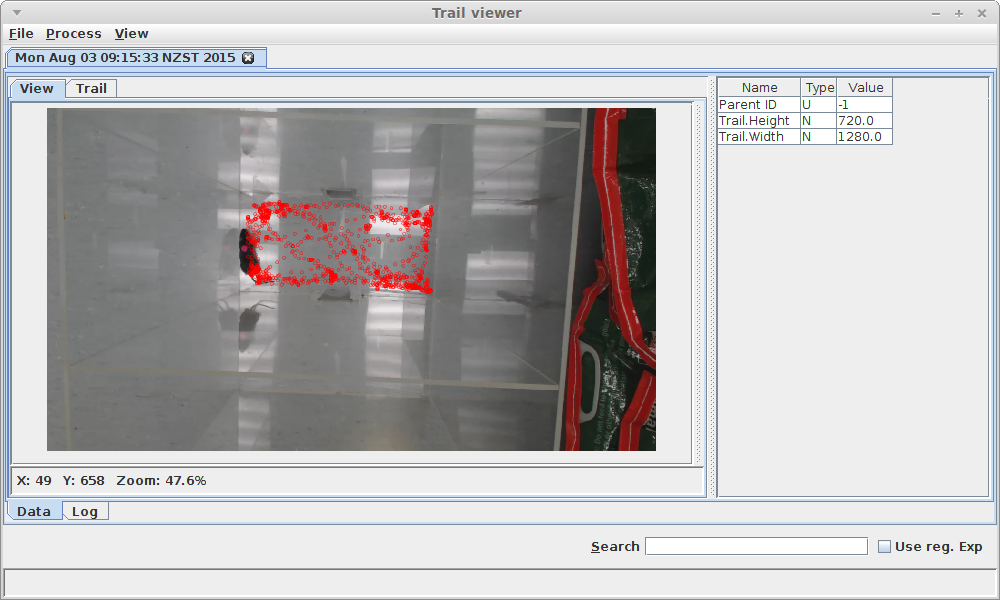
\includegraphics[width= 12.0cm]{images/trail_viewer.png}
  \caption{Annotator showing a video and key shortcuts}
  \label{annotator_in_use}
\end{figure}

%%%%%%%%%%%%%%%%%%%%%%%%%%%%%%%%%%%
\section{Annotator}

The annotator has three menus which we will cover in the following sections.

\begin{figure}[htb]
  \centering
  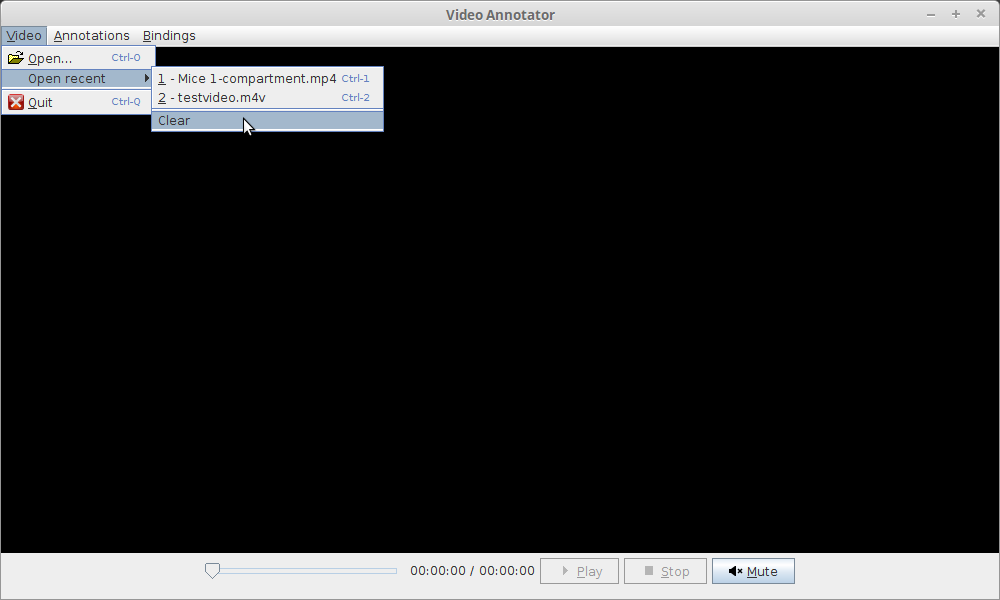
\includegraphics[width=12.0cm]{images/AnnotatorVideoMenu.png}
  \caption{Video menu.}
  \label{AnnotatorVideoMenu}
\end{figure}

\subsection{Video Menu}
The video menu (see Figure \ref{AnnotatorVideoMenu}) lets you open video
files or quit the program. It also provides a list of recently opened videos.

\begin{figure}[htb]
  \centering
  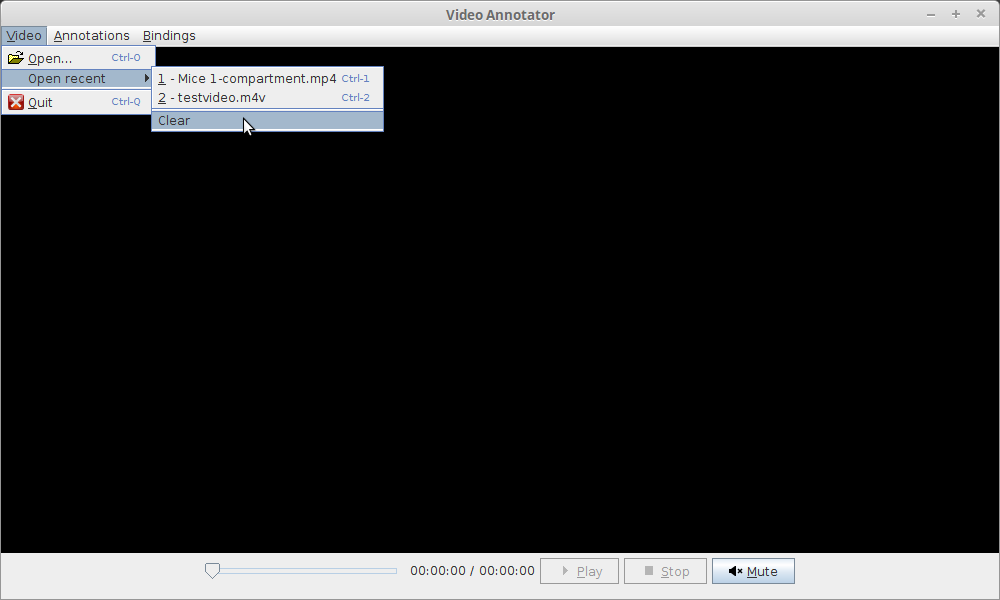
\includegraphics[width=12.0cm]{images/AnnotatorVideoMenu.png}
  \caption{Video menu.}
  \label{AnnotatorVideoMenu}
\end{figure}

\subsection{Annotations Menu}
This menu lets you create a new set of annotations or export the current
set to a spreadsheet file, e.g., CSV or, depending on modules present,
MS Excel (see Figure \ref{AnnotatorAnnotationMenu}).

\begin{figure}[htb]
  \centering
  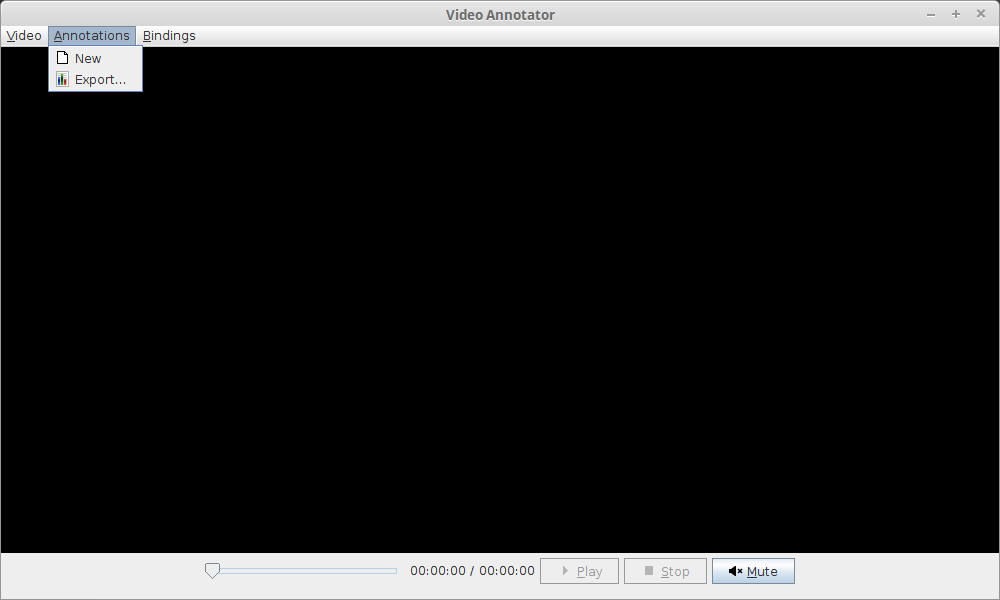
\includegraphics[width=12.0cm]{images/AnnotatorAnnotationMenu.png}
  \caption{Annotations menu.}
  \label{AnnotatorAnnotationMenu}
\end{figure}

\subsection{Background Menu}
The background menu, as depicted in Figure \ref{AnnotatorBackgroundMenu} allows for the extraction of the background
of a video. This requires that the camera shooting the video was fixed. The menu alows you to clear the current
background, extract the background from the currently loaded video, save or load the background, and view the
current background iamge.


\begin{figure}[htb]
  \centering
  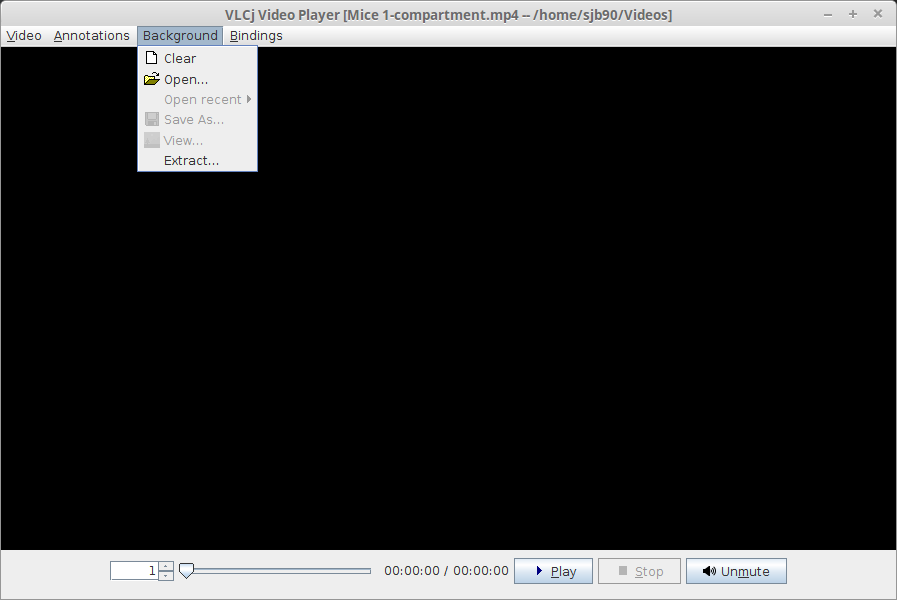
\includegraphics[width=12.0cm]{images/AnnotatorBackgroundMenu.png}
  \caption{Background menu.}
  \label{AnnotatorBackgroundMenu}
\end{figure}

\subsection{Extract Background}
Extracting the background is done in the dialog seen in Figure \ref{AnnotatorExtractBackground}.

\begin{figure}[htb]
  \centering
  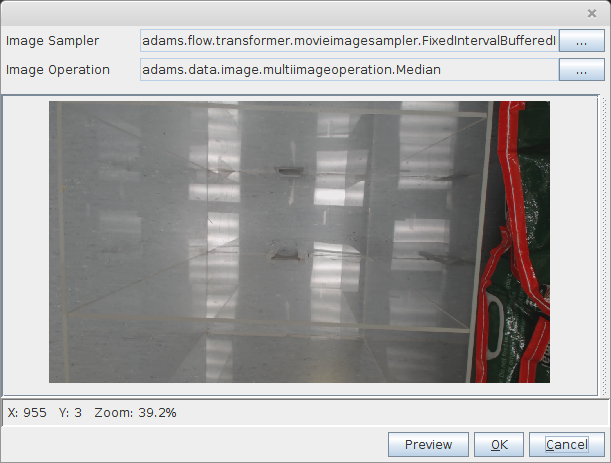
\includegraphics[width=12.0cm]{images/AnnotatorExtractBackground.png}
  \caption{Extract Background Dialog}
  \label{AnnotatorExtractBackground}
\end{figure}

Here a user can select an image sampler and image operation to use to generate the background. Usually the defaults
should be sufficient. The selection process can be seen in Figure \ref{AnnotatorSamplerSelection}.

\begin{figure}[htb]
  \centering
  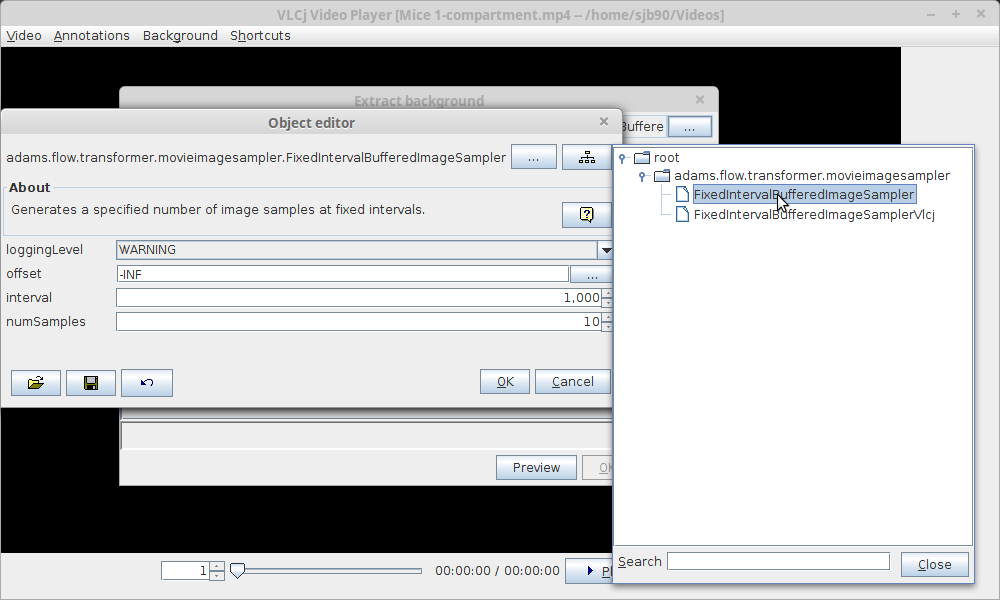
\includegraphics[width=12.0cm]{images/AnnotatorBackgroundExtractionSamplerSelection.png}
  \caption{Extract Background Dialog}
  \label{AnnotatorSamplerSelection}
\end{figure}

\subsection{Shortcuts Menu}
The shortcuts menu, as depicted in Figure \ref{AnnotatorShortcutsMenu}, allows
for the creation of a new set of shortcuts, loading or saving shortcuts, and
editing the current shortcuts.

\begin{figure}[htb]
  \centering
  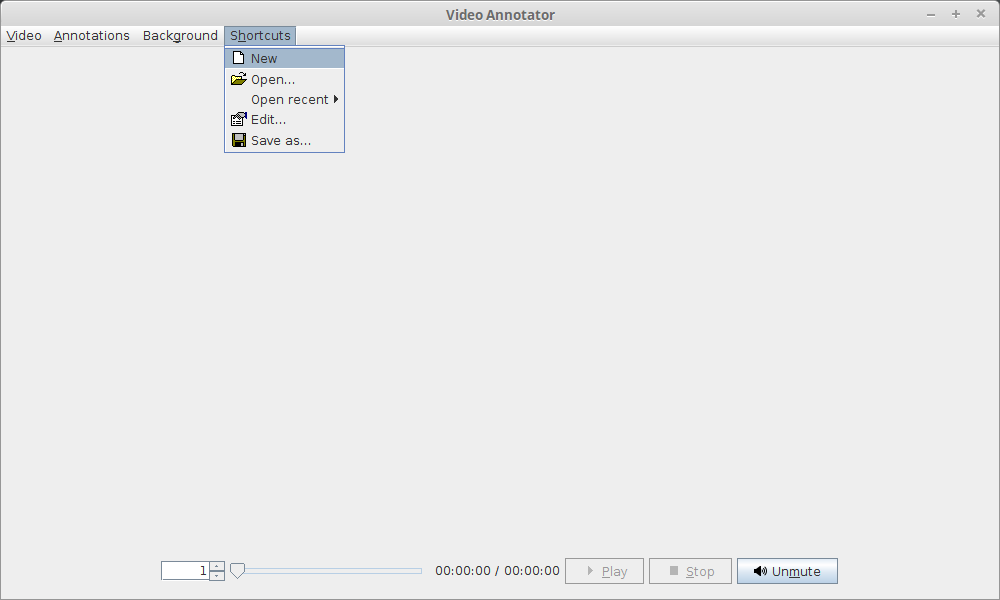
\includegraphics[width=12.0cm]{images/AnnotatorShortcutsMenu.png}
  \caption{Shortcuts menu.}
  \label{AnnotatorShortcutsMenu}
\end{figure}

\subsubsection{Edit Shortcuts}
When editing shortcuts you can add new shortcuts, edit a current shortcut or
remove selected shortcuts (see Figure \ref{AnnotationEditShortcuts}).

\begin{figure}[htb]
  \centering
  \includegraphics[width=7.0cm]{images/AnnotationEditShortcuts.png}
  \caption{Edit shortcuts dialog.}
  \label{AnnotationEditShortcuts}
\end{figure}

When editing a shortcut there are various options for customizing the output
from the shortcut.

The output from a shortcut is made up of a header and \textit{true} or
\textit{false} along with a timestamp:

\begin{verbatim}
Timestamp,Meta-Shortcut1,Meta-Shortcut2
00:00:00.000,false,false
00:00:01.000,false,true
\end{verbatim}

In this case the name of the shortcut shows up as \textit{Shortcut1} and
\textit{Shortcut2}. Figure \ref{AnnotatorAddShortcut} shows the dialog for editing a
shortcut.

\begin{figure}[htb]
  \centering
  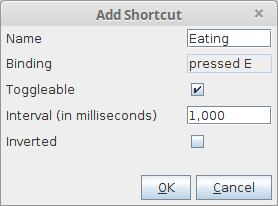
\includegraphics[width=4.0cm]{images/AnnotatorAddShortcut.png}
  \caption{Dialog for editing a shortcut.}
  \label{AnnotatorAddShortcut}
\end{figure}

In the following, an description of what each of the shortcut parameters is
used for:
\begin{tight_itemize}
  \item \textbf{Name} -- This is what gets output as the header of the
  annotation file when it is exported
  \item \textbf{Shortcut} -- The key for this shortcut. It is entered by
  selecting the text box and then pressing the desired key or key combination
  -- i.e. \texttt{ctrl + B} or just \texttt{B}
  \item \textbf{Toggleable} -- If this is checked then the shortcut always
  outputs a value, usually \textit{false}, and when it is toggled switches
  that output to \textit{true}.
  \item \textbf{Interval} -- Only relevant for toggleable shortcuts. This is
  the interval at which the values will be output. By default it is 1,000
  milliseconds (= 1 second) but it can be changed to any number. Intervals
  below 1 second tend to become less accurate, so if set at 10 ms it might
  output a value between 1 - 20 ms rather than 10 depending on CPU load and
  scheduling. It is recommended to use times of a second or above.
  \item \textbf{Inverted} -- This allows you to invert the values output
  by the shortcut. Usually a shortcut outputs \textit{true} when pressed or, in the
  case of toggleable shortcuts, toggled on. This will invert that so when
  it is pressed it will output \textit{false} and in the case of a toggleable it
  will output a value of \textit{true} when it is toggled off and \textit{false} when toggled on.
\end{tight_itemize}


%%%%%%%%%%%%%%%%%%%%%%%%%%%%%%%%%%%
\chapter{Data}
\section{.trail format}
The \textit{.trail} format is a simple text format. In its essence it is
spreadsheet-like format with a header and a body.

The \textit{header} contains the meta-data for the trail. Most importantly,
the width and the height of the trail. The format is in Java Properties format,
each line prefixed with ``\# ''. Each stored value also defines in a separate
property what data type it is (N = numeric, S = string, B = boolean).

It is possible to store an optional background image in the header. The image
data is stored as RGBA signed bytes, row-by-row. In order to produce smaller
files, the data is compressed using gzip\cite{gzip}. The compressed bytes are
then stored in a upper-case hexadecimal notation, with a maximum of 1000 bytes
per line. The background data lines are prefixed with ``\% ''.

The \textit{body} consists of four columns: timestamp (with milli-seconds), X position,
Y position, meta-data for that step. The meta-data column is a blank-separated list of
key-value pairs (``key=value"").

Here is an example file, without a background:

\begin{verbatim}
# #Tue Jul 28 09:24:20 NZST 2015
# Trail.Height\tDataType=N
# Trail.Width\tDataType=N
# Trail.Height=720.0
# Parent\ ID=-1
# Trail.Width=1280.0
Timestamp,X,Y,Meta-data
"00:00:00.127",424,292,""
"00:00:00.224",423,285,""
"00:00:00.304",423,277,""
\end{verbatim}


%%%%%%%%%%%%%%%%%%%%%%%%%%%%%%%%%%%
\chapter{Video Annotator}
\section{Useage}
The annotator has three menus which we will cover here

%%%%%%%%%%%%%%%%%%%%%%%%%%%%%%%%%%%
% Copyright (c) 2009-2012 by the University of Waikato, Hamilton, NZ. 
% This work is made available under the terms of the 
% Creative Commons Attribution-ShareAlike 4.0 license,
% http://creativecommons.org/licenses/by-sa/4.0/.
%
% Version: $Revision$

\begin{thebibliography}{999}
	% to make the bibliography appear in the TOC
	\addcontentsline{toc}{chapter}{Bibliography}

    % references
	\bibitem{adams}
		\textit{ADAMS} -- Advanced Data mining and Machine learning System \\
		\url{https://adams.cms.waikato.ac.nz/}{}
		
	\bibitem{heatmap}
		\textit{Heat map} -- WikiPedia article \\
		\url{http://en.wikipedia.org/wiki/Heat_map}{}

\end{thebibliography}


\end{document}
